Para estimar el coste de una batería de tipo LiFePO4 (Lithium Iron Phosphate)
por $kWh$ de capacidad, hemos recopilado información para varios modelos
comerciales \footnote{disponibles a la venta en
\url{https://autosolar.es/baterias-de-litio} y
\url{https://www.tesla.com/es_es/powerwall/get}} visibles en la tabla
\ref{tab:batteries_data}.

\begin{table}[htbp]
	\centering
	\begin{tabular}{llrrr}
		\toprule
		Marca     & Modelo            & kWh   & Precio (€) & € / kWh \\
		\midrule
		upower    & UE-12Li50BL       & 0.64  & 222.64     & 347.88  \\
		upower    & UE-FT-12Li100     & 1.28  & 461.00     & 360.16  \\
		tesla     & powerwall         & 13.00 & 7000.00    & 538.46  \\
		Pylontech & RT12100G31        & 1.28  & 689.00     & 538.28  \\
		Victron   & LFPSmart/12,8/50  & 0.64  & 779.00     & 1217.19 \\
		Victron   & LFPSmart/12,8/180 & 2.30  & 1084.00    & 470.49  \\
		Victron   & LFPSmart/25.6/100 & 2.56  & 2120.00    & 828.13  \\
		Victron   & LFPSmart/25.6/200 & 5.12  & 2265.00    & 442.38  \\
		Huawei    & luna2000          & 5.00  & 2679.00    & 535.80  \\
		Pylontech & Force L1          & 7.10  & 2900.00    & 408.45  \\
		BYD       & Premium LVS/4kWh  & 4.00  & 2600.00    & 650.00  \\
		Growatt   & ARK SPH TL3       & 7.60  & 4800.00    & 631.58  \\
		Pylontech & Force L2          & 14.20 & 5670.00    & 399.30  \\
		LG        & HBC               & 15.80 & 6992.00    & 442.53  \\
		LG        & Resu 10H Prime    & 9.80  & 8600.00    & 877.55  \\
		SolarEdge & Energy bank       & 10.00 & 9893.00    & 989.30  \\
		BYD       & B-Box Premium LVS & 24.00 & 16500.00   & 687.50  \\
		BYD       & B-Box HVM Premium & 22.10 & 11980.00   & 542.08  \\
		LG        & Resu 16H Prime    & 16.00 & 12360.00   & 772.50  \\
		\bottomrule
	\end{tabular}
	\caption{Comparison of Energy Storage Systems by Brand and Model}
	\label{tab:batteries_data}
\end{table}

Y posteriormente ajustando por regresión lineal la ecuación para el coste por
unidad de capacidad:

\begin{equation}
	\text{coste\_baterias} \left[\frac{\text{\euro}}{kWh}\right] = 11.87 + 611.78 \cdot e_{\text{bat\_max}}
\end{equation}

donde $e_{\text{bat\_max}}$ es la capacidad de la batería en $kWh$, y en la
figura \ref{fig:batteries_regression} se muestran los puntos de información y
la aproximación.

\begin{figure}[h] \centering
	\centering
	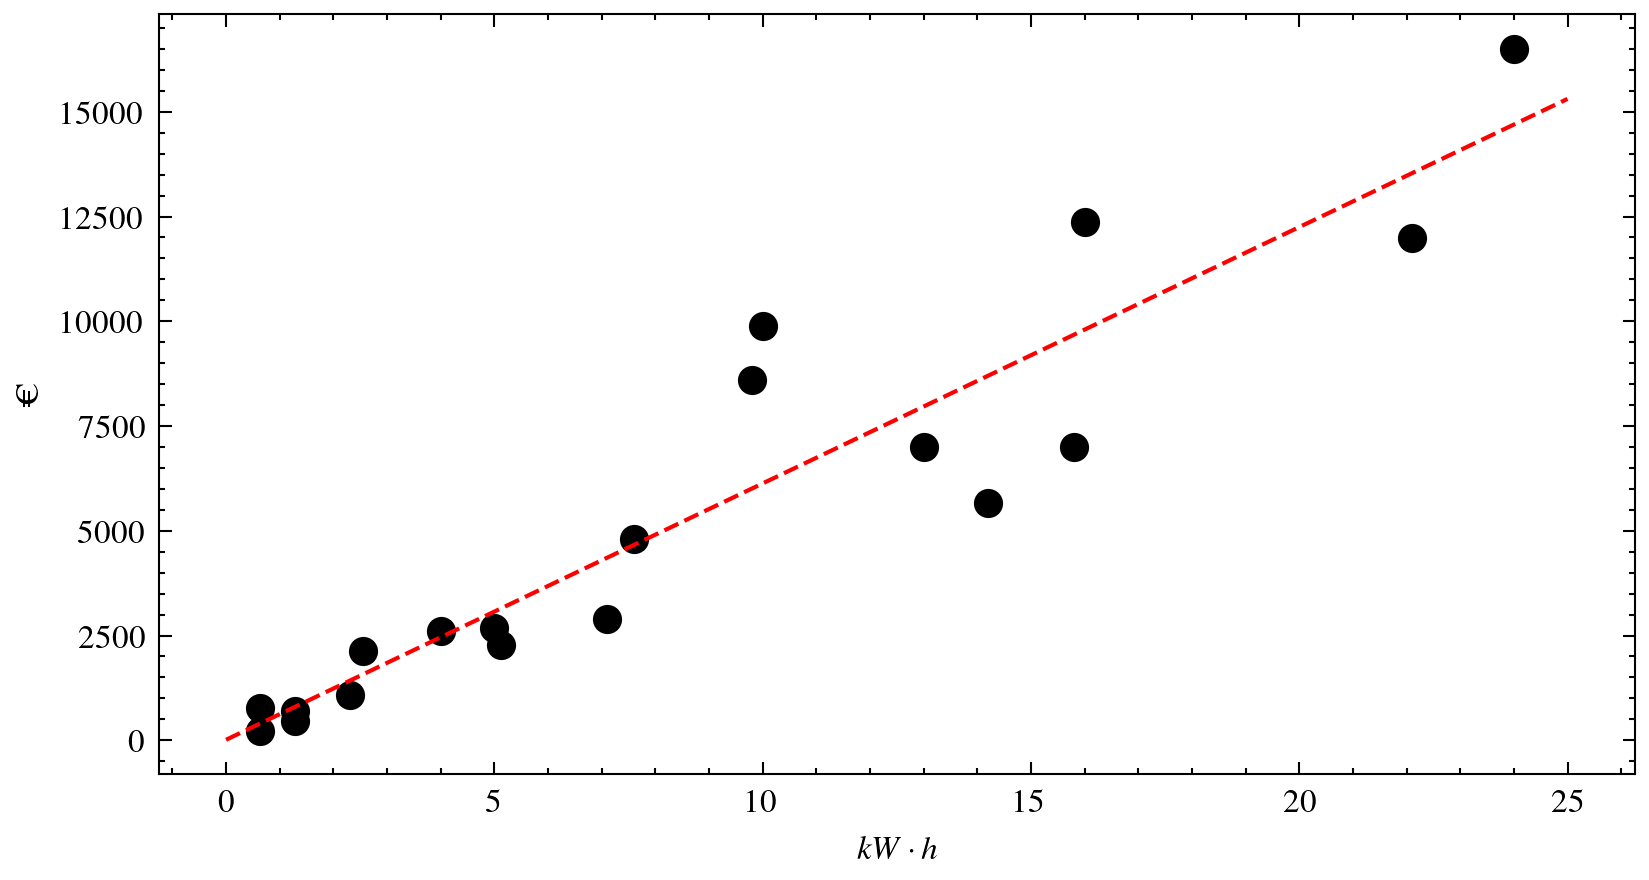
\includegraphics[width=1\textwidth]{./capitulos/adquisicion_de_datos/images/batteries_regression.png}
	\caption{Ajuste lineal de precios para baterías LiFePO4.}
	\label{fig:batteries_regression}
\end{figure}
